\documentclass[11pt,a4paper]{article}

\usepackage[utf8]{inputenc}
\usepackage[T1]{fontenc}
\usepackage[margin=1in]{geometry}
\usepackage{amsmath,amssymb,amsfonts}
\usepackage{graphicx}
\usepackage{xcolor}
\usepackage{booktabs}
\usepackage{tabularx}
\usepackage{array}
\usepackage{listings}
\usepackage{tikz}
\usetikzlibrary{shapes.geometric, arrows.meta, positioning, calc, fit}
\usepackage{enumitem}
\usepackage{caption}
\usepackage{subcaption}
\usepackage{float}
\usepackage{hyperref}

\hypersetup{
    colorlinks=true,
    linkcolor=black,
    citecolor=black,
    urlcolor=blue!70!black,
    pdftitle={Telnet Remote-Management Lab},
    pdfauthor={Subham Bhat}
}

\definecolor{codebg}{rgb}{0.96,0.96,0.96}
\definecolor{codeframe}{rgb}{0.25,0.25,0.25}
\definecolor{codenum}{rgb}{0.45,0.45,0.45}

\lstset{
    backgroundcolor=\color{codebg},
    basicstyle=\ttfamily\footnotesize,
    breakatwhitespace=false,
    breaklines=true,
    captionpos=b,
    commentstyle=\color{codenum}\itshape,
    keywordstyle=\bfseries,
    numberstyle=\tiny\color{codenum},
    numbers=left,
    numbersep=8pt,
    frame=single,
    rulecolor=\color{codeframe},
    tabsize=4,
    columns=flexible,
    keepspaces=true,
    showspaces=false,
    showstringspaces=false,
    xleftmargin=14pt,
    xrightmargin=4pt,
    literate={→}{{$\rightarrow$}}1 {←}{{$\leftarrow$}}1 {–}{{--}}1 {—}{{---}}1 {·}{{$\cdot$}}1 {✓}{{OK}}2 {✗}{{X}}1
}

\newcolumntype{Y}{>{\raggedright\arraybackslash}X}

% screenshot from docs/screenshots (skipped quietly if the file is missing)
\newcommand{\shot}[3][0.92\textwidth]{%
  \IfFileExists{docs/screenshots/#2}{%
  \begin{figure}[H]\centering
  \includegraphics[width=#1,keepaspectratio]{docs/screenshots/#2}
  \caption{#3}\end{figure}}{}}

\emergencystretch=3em
\setlength{\parindent}{1.5em}
\setlength{\parskip}{0.4em}

\begin{document}

% ==============================================================================
% TITLE PAGE
% ==============================================================================
\begin{titlepage}
    \centering
    \vspace*{4.2cm}

    {\LARGE \textbf{Telnet Remote-Management Lab: RFC 854 NVT,}}\\[0.7em]
    {\LARGE \textbf{RFC 1143 Option Negotiation, IOS-Style VTY}}\\[0.7em]
    {\LARGE \textbf{Server, and Plaintext vs TLS Sniffing}}\\[1.4em]

    {\large for Computer Networks Laboratory}

    \vspace{3.8cm}

    {\large
    \textbf{Name:} Subham Bhat\\[0.55em]
    \textbf{Class:} BCSE III\\[0.55em]
    \textbf{Roll:} 002410501020\\[0.55em]
    \textbf{Group:} A1\\[0.55em]
    \textbf{College:} Jadavpur University
    }

    \vfill
    {\normalsize 1}
\end{titlepage}

% ==============================================================================
% TABLE OF CONTENTS
% ==============================================================================
\pagenumbering{roman}
\setcounter{page}{2}
\tableofcontents
\newpage

% ==============================================================================
% MAIN CONTENT
% ==============================================================================
\pagenumbering{arabic}
\setcounter{page}{3}

\section{Introduction}
\noindent Remote log-in lets a user at one machine work on another as if the keyboard and screen were attached to it directly. The oldest standard for this on the Internet is \textbf{TELNET} (\textbf{TEL}etype \textbf{NET}work), specified in \textbf{RFC 854} (1983). It runs over \textbf{TCP port 23} and is still used to manage routers and switches on isolated lab networks, which is exactly how router \texttt{JU-Main-R} was configured in Assignment~6.

Telnet has three ideas worth studying:
\begin{itemize}[leftmargin=2em]
    \item \textbf{The Network Virtual Terminal (NVT):} both ends translate their local character set into one agreed 7-bit ASCII representation with fixed end-of-line rules, so neither side needs to know the other's terminal.
    \item \textbf{In-band commands:} control functions (Interrupt Process, Erase Character, Are You There, \ldots) and option negotiation travel in the same TCP byte stream as the data, introduced by the escape byte \textbf{IAC = 255}.
    \item \textbf{Symmetric option negotiation:} either side may offer or request features such as remote echo or window-size reporting with \texttt{WILL}, \texttt{WONT}, \texttt{DO} and \texttt{DONT}. A careless implementation can loop forever; \textbf{RFC 1143} (the ``Q method'') fixes this.
\end{itemize}

Its weakness is equally instructive: \textbf{everything, including the password, crosses the network in clear text}. This is why SSH replaced it.

\subsection{What Was Built}
This module is a complete Telnet laboratory written from the RFCs in pure Java 11 with no external libraries:
\begin{enumerate}[leftmargin=2em]
    \item \textbf{Protocol engine} (\texttt{telnet.protocol}): an RFC 854 NVT codec implemented as a state machine, and an RFC 1143 option negotiator for ECHO, SUPPRESS-GO-AHEAD, STATUS, TIMING-MARK, TERMINAL-TYPE, NAWS and TERMINAL-SPEED.
    \item \textbf{Server} (\texttt{telnet.server}): the five VTY lines of router \texttt{JU-Main-R} (\texttt{line vty 0 4}), character-at-a-time mode with server-side echo, and a Cisco IOS-style command shell with user, privileged and configuration modes, abbreviations, \texttt{?} help and Tab completion.
    \item \textbf{Client} (\texttt{telnet.client}): a console Telnet client that negotiates the same options.
    \item \textbf{Wire tap} (\texttt{telnet.tap}): a man-in-the-middle relay that shows exactly what a sniffer on the path sees, including the reconstructed password.
    \item \textbf{Telnet over TLS} (``telnets'') on a second port, and a \textbf{brute-force guard} modelled on IOS \texttt{login block-for}.
    \item \textbf{Live dashboard} on \texttt{http://localhost:8081} that follows the lecture slides chapter by chapter.
\end{enumerate}

\begin{table}[H]
\centering
\caption{Ports used by the Telnet module}
\small
\begin{tabularx}{\textwidth}{@{}llY@{}}
\toprule
\textbf{Port} & \textbf{Protocol} & \textbf{Role} \\ \midrule
TCP 2323 & Telnet & The server (real port 23 needs administrator rights on Windows). \\
TCP 2324 & Telnet & Wire tap relaying to 2323: shows what a sniffer sees. \\
TCP 9923 & Telnet over TLS & ``telnets'' (real port 992) with a self-signed certificate made by \texttt{keytool}. \\
TCP 9924 & TLS & Wire tap relaying to 9923: shows that TLS hides everything. \\
HTTP 8081 & HTTP & The dashboard. \\ \bottomrule
\end{tabularx}
\end{table}

\shot{01_remote_login_and_terminal.png}{Chapter 01 of the dashboard: the remote log-in path from the lecture slides, with a live browser terminal.}

% ==============================================================================
\section{The Protocol}

\subsection{Local and Remote Log-in}
On a local log-in, keystrokes go from the terminal to the \emph{terminal driver} of the operating system, which hands them to the shell. On a remote log-in, the Telnet \emph{client} takes them from the terminal driver, converts them to NVT form and sends them over TCP. On the server, the Telnet \emph{server} cannot hand bytes to the shell directly, because the shell expects a terminal. A \textbf{pseudo-terminal driver} sits in between and makes the shell believe a real terminal is attached.

\begin{figure}[H]
\centering
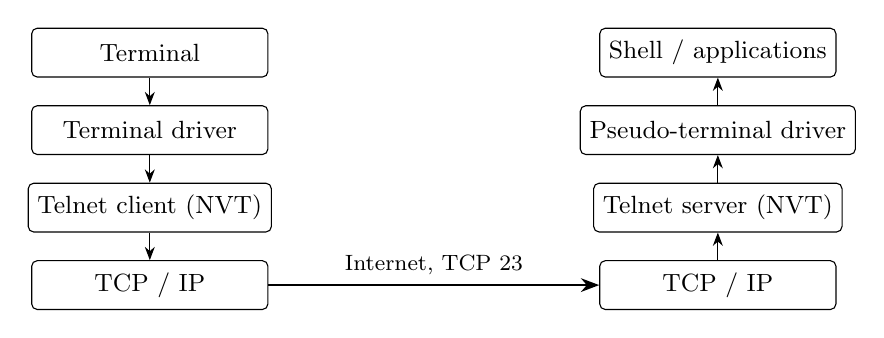
\begin{tikzpicture}[node distance=0.35cm, box/.style={draw, rounded corners=2pt, minimum width=3.0cm, minimum height=0.62cm, font=\small}, >=Stealth]
\node[box] (t) {Terminal};
\node[box, below=of t] (td) {Terminal driver};
\node[box, below=of td] (tc) {Telnet client (NVT)};
\node[box, below=of tc] (tcp1) {TCP / IP};
\node[box, right=4.2cm of t] (sh) {Shell / applications};
\node[box, below=of sh] (pty) {Pseudo-terminal driver};
\node[box, below=of pty] (ts) {Telnet server (NVT)};
\node[box, below=of ts] (tcp2) {TCP / IP};
\draw[->] (t) -- (td); \draw[->] (td) -- (tc); \draw[->] (tc) -- (tcp1);
\draw[->] (tcp2) -- (ts); \draw[->] (ts) -- (pty); \draw[->] (pty) -- (sh);
\draw[->, thick] (tcp1.east) -- node[above, font=\footnotesize]{Internet, TCP 23} (tcp2.west);
\end{tikzpicture}
\caption{Remote log-in: the path of every keystroke and echo.}
\end{figure}

\subsection{The Network Virtual Terminal and Its Commands}
NVT data characters are 7-bit ASCII with the most significant bit 0. End of line is always \texttt{CR LF}; a bare carriage return is sent as \texttt{CR NUL}. Control is signalled in-band: the byte \textbf{IAC (255)} means ``the next byte is a command''. A data byte that happens to be 255 is therefore sent twice (\texttt{FF FF}).

\begin{table}[H]
\centering
\caption{Telnet commands (RFC 854) implemented by the codec}
\small
\begin{tabularx}{\textwidth}{@{}llY@{}}
\toprule
\textbf{Name} & \textbf{Code} & \textbf{Meaning} \\ \midrule
SE / SB & 240 / 250 & End / begin of sub-negotiation (\texttt{IAC SB option \ldots{} IAC SE}). \\
NOP, DM, BRK & 241, 242, 243 & No operation, data mark (for urgent data), break. \\
IP, AO, AYT & 244, 245, 246 & Interrupt process, abort output, \emph{Are You There?} \\
EC, EL, GA & 247, 248, 249 & Erase character, erase line, go ahead. \\
WILL, WONT & 251, 252 & ``I will (will not) enable this option on my side.'' \\
DO, DONT & 253, 254 & ``Please (do not) enable this option on your side.'' \\
IAC & 255 & Interpret As Command; doubled when it is a data byte. \\ \bottomrule
\end{tabularx}
\end{table}

A command sequence on the wire therefore looks like \texttt{[IAC][DO][ECHO]} = \texttt{FF FD 01}. Sub-negotiation carries values, for example the terminal type:
\begin{center}\texttt{[IAC][SB][24][IS]'x''t''e''r''m'[IAC][SE]}\end{center}

\subsection{Options}
\begin{table}[H]
\centering
\caption{Options negotiated by the server and client}
\small
\begin{tabularx}{\textwidth}{@{}llcY@{}}
\toprule
\textbf{Option} & \textbf{RFC} & \textbf{Code} & \textbf{Use in this lab} \\ \midrule
ECHO & 857 & 1 & The server echoes; the password is simply not echoed. \\
SUPPRESS-GO-AHEAD & 858 & 3 & Together with ECHO this gives character-at-a-time mode. \\
STATUS & 859 & 5 & \texttt{IAC SB STATUS SEND} returns the options the server believes are on. \\
TIMING-MARK & 860 & 6 & Used by \texttt{tmping} to measure round-trip time. \\
TERMINAL-TYPE & 1091 & 24 & The client's type list is cycled until it repeats. \\
NAWS & 1073 & 31 & Window size; the full-screen \texttt{top} command reflows on resize. \\
TERMINAL-SPEED & 1079 & 32 & Reported by the client. \\
BINARY, LINEMODE, \ldots & & & Refused correctly with \texttt{WONT} / \texttt{DONT}. \\ \bottomrule
\end{tabularx}
\end{table}

% ==============================================================================
\section{System Architecture}

\begin{figure}[H]
\centering
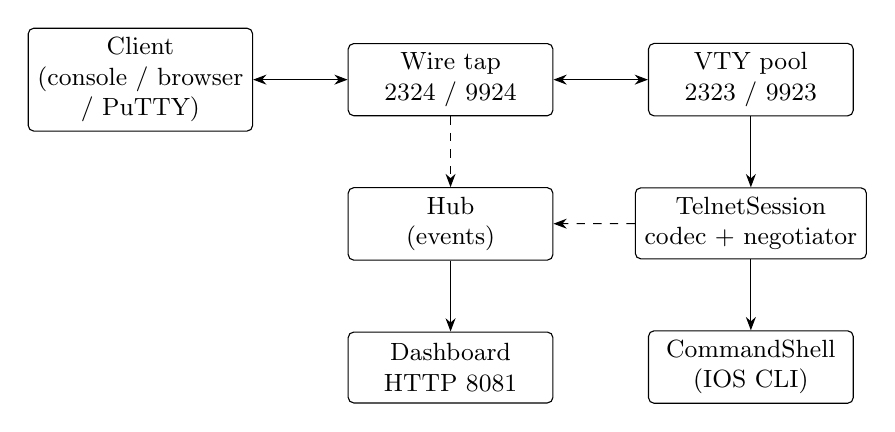
\begin{tikzpicture}[node distance=1.0cm, box/.style={draw, rounded corners=2pt, minimum width=2.6cm, minimum height=0.9cm, align=center, font=\small}, >=Stealth]
\node[box] (cl) {Client\\(console / browser\\/ PuTTY)};
\node[box, right=1.2cm of cl] (tap) {Wire tap\\2324 / 9924};
\node[box, right=1.2cm of tap] (srv) {VTY pool\\2323 / 9923};
\node[box, below=0.9cm of srv] (sess) {TelnetSession\\codec + negotiator};
\node[box, below=0.9cm of sess] (sh) {CommandShell\\(IOS CLI)};
\node[box, below=0.9cm of tap] (hub) {Hub\\(events)};
\node[box, below=0.9cm of hub] (dash) {Dashboard\\HTTP 8081};
\draw[<->] (cl) -- (tap); \draw[<->] (tap) -- (srv); \draw[->] (srv) -- (sess); \draw[->] (sess) -- (sh);
\draw[->, dashed] (tap) -- (hub); \draw[->, dashed] (sess) -- (hub); \draw[->] (hub) -- (dash);
\end{tikzpicture}
\caption{Components of the Telnet module.}
\end{figure}

\begin{table}[H]
\centering
\caption{Source files}
\small
\begin{tabularx}{\textwidth}{@{}lY@{}}
\toprule
\textbf{Package / file} & \textbf{Responsibility} \\ \midrule
\texttt{protocol/Telnet.java} & Command and option constants with names. \\
\texttt{protocol/TelnetCodec.java} & RFC 854 decoder state machine and encoder. \\
\texttt{protocol/OptionNegotiator.java} & RFC 1143 Q-method, every message labelled with its textbook meaning. \\
\texttt{protocol/LoopExperiment.java} & Naive vs Q-method negotiation experiment. \\
\texttt{server/VtyPool.java} & Five VTY lines; a sixth connection is refused. \\
\texttt{server/TelnetSession.java} & One VTY line: login, line editor, history, options. \\
\texttt{server/CommandShell.java} & IOS-style command tree and modes. \\
\texttt{server/DeviceConfig.java} & Users, PBKDF2 secrets, \texttt{login block-for}, \texttt{write memory}. \\
\texttt{server/LoginGuard.java} & Brute-force detection and quiet mode. \\
\texttt{tap/WireTap.java} & Sniffing relay and credential reconstruction. \\
\texttt{client/TelnetClient.java} & Console client. \\
\texttt{dashboard/DashboardServer.java} & HTTP API, browser-terminal bridge, attack bot. \\ \bottomrule
\end{tabularx}
\end{table}

% ==============================================================================
\section{Implementation}

\subsection{The NVT Codec as a State Machine}
TCP is a byte stream with no message boundaries, so a command can be split across two reads: \texttt{FF} at the end of one segment and \texttt{FD 1F} at the start of the next. A decoder that looks at whole buffers fails on such input. The codec therefore keeps its state between calls and consumes one byte at a time.

\begin{lstlisting}[language=Java, caption={The RFC 854 decoder in \texttt{TelnetCodec.java}.}]
private enum State { DATA, IAC, NEGOTIATE, SB_OPTION, SB_DATA, SB_IAC }

public void feed(int b) {
    switch (state) {
        case DATA:
            if (b == Telnet.IAC) state = State.IAC;
            else listener.onData(b);
            break;
        case IAC:
            if (b == Telnet.IAC) { listener.onData(Telnet.IAC); state = State.DATA; }   // escaped 255
            else if (b >= Telnet.WILL && b <= Telnet.DONT) { verb = b; state = State.NEGOTIATE; }
            else if (b == Telnet.SB) { state = State.SB_OPTION; }
            else { listener.onCommand(b); state = State.DATA; }                    // AYT, IP, EC ...
            break;
        case NEGOTIATE:
            listener.onNegotiation(verb, b);
            state = State.DATA;
            break;
        case SB_OPTION: sbOption = b; sb.reset(); state = State.SB_DATA; break;
        case SB_DATA:
            if (b == Telnet.IAC) state = State.SB_IAC; else sb.write(b);
            break;
        case SB_IAC:
            if (b == Telnet.SE) { listener.onSubnegotiation(sbOption, sb.toByteArray()); state = State.DATA; }
            else if (b == Telnet.IAC) { sb.write(Telnet.IAC); state = State.SB_DATA; }
            else { state = State.DATA; }   // malformed: drop the sub-negotiation
            break;
    }
}

/** Escape user data for the wire: 0xFF -> FF FF, bare CR -> CR NUL. */
public static byte[] encodeData(byte[] data) {
    ByteArrayOutputStream out = new ByteArrayOutputStream(data.length + 8);
    for (int i = 0; i < data.length; i++) {
        int b = data[i] & 0xFF;
        out.write(b);
        if (b == Telnet.IAC) out.write(Telnet.IAC);
        if (b == '\r' && (i + 1 >= data.length || data[i + 1] != '\n')) out.write(0);
    }
    return out.toByteArray();
}
\end{lstlisting}

The verification suite feeds the same byte stream through the decoder in \textbf{2000 random segmentations} and checks that every one decodes identically.

\textbf{Embedding a command in data.} The textbook example sends \texttt{c a t \_ f i l e a IAC EC 1} as one TCP segment. The server's line editor applies the Erase Character command in place, so the command that runs is \texttt{cat file1}. The dashboard has a button that sends exactly this segment.

\subsection{Option Negotiation: Why a Naive Implementation Loops}
The simple rule ``answer every \texttt{DO} with \texttt{WILL}'' breaks when both sides change their mind at the same time: each acknowledges the other's request with a new request, and the messages bounce forever. RFC 1143 gives each side, for each option, one of four states (\texttt{NO}, \texttt{YES}, \texttt{WANTNO}, \texttt{WANTYES}) plus a one-bit queue. A side never replies to a message that only confirms its current state, so the exchange always terminates.

\begin{lstlisting}[language=Java, caption={Receiving WILL under the Q method (\texttt{OptionNegotiator.java}).}]
private void recvWill(int o) {
    Q b = him[o];
    switch (b) {
        case NO:
            if (policy.acceptRemote(o)) { him[o] = Q.YES; send(Telnet.DO, o, APPROVE_OFFER_EN); changed(false, o, true); }
            else { send(Telnet.DONT, o, DISAPPROVE_OFFER_EN); }        // refuse the offer
            break;
        case YES:   break;                                          // already on: no reply, so no loop
        case WANTNO:
            if (!himQueue[o]) him[o] = Q.NO;                         // error: DONT answered by WILL
            else { him[o] = Q.YES; himQueue[o] = false; }
            break;
        case WANTYES:
            if (!himQueue[o]) { him[o] = Q.YES; changed(false, o, true); }   // our DO acknowledged
            else { him[o] = Q.WANTNO; himQueue[o] = false; send(Telnet.DONT, o, REQ_DIS); }
            break;
    }
}
\end{lstlisting}

Every message is also labelled with the meaning it has in the textbook table. The same byte \texttt{IAC WILL ECHO} is ``\emph{Offering to enable}'' when the sender was in state \texttt{NO}, but ``\emph{Accepting a request to enable}'' when it answers our \texttt{DO}. The dashboard shows these labels on the live session.

\shot[0.85\textwidth]{05_negotiation_meanings.png}{Chapter 05: every WILL/WONT/DO/DONT of the opening negotiation, labelled with its textbook meaning.}

\textbf{The loop experiment.} \texttt{LoopExperiment.java} connects two endpoints and makes both change their ECHO setting at the same moment. With naive endpoints the messages never stop (the run is cut at a cap); with RFC 1143 endpoints the exchange finishes in \textbf{4 messages} and both ends agree on the final state.

\shot[0.85\textwidth]{08_rfc1143_loop_experiment.png}{The naive endpoints loop until the cap; the Q-method converges in four messages.}

\subsection{The Server: VTY Lines and an IOS-Style Shell}
\texttt{VtyPool} accepts at most five concurrent sessions, like \texttt{line vty 0 4}; the sixth connection receives a refusal message and is closed. Each \texttt{TelnetSession} starts by offering \texttt{WILL ECHO} and \texttt{WILL SUPPRESS-GO-AHEAD} and asking \texttt{DO TERMINAL-TYPE}, \texttt{DO NAWS} and \texttt{DO TERMINAL-SPEED}. With server echo and no go-ahead, every keystroke is sent as soon as it is typed and the server decides what to echo. At the \texttt{Password:} prompt it echoes nothing.

The shell implements the IOS command tree with abbreviations (\texttt{sh ip int br}), context help with \texttt{?}, Tab completion, \texttt{\% Invalid input} with a \texttt{\^{}} marker, user EXEC (\texttt{>}), privileged EXEC (\texttt{\#}) and configuration modes, \texttt{enable}, \texttt{configure terminal}, \texttt{hostname}, \texttt{banner motd}, \texttt{username \ldots{} secret}, \texttt{exec-timeout}, \texttt{write memory}, \texttt{show users}, \texttt{show telnet} (the live RFC 1143 state of each option), \texttt{tmping} (RTT via TIMING-MARK) and a full-screen \texttt{top} that redraws when NAWS reports a new window size. Passwords are stored as \textbf{PBKDF2-SHA256} hashes (Cisco type 8) and compared in constant time.

\begin{table}[H]
\centering
\caption{Accounts configured on the router}
\small
\begin{tabular}{@{}lll@{}}
\toprule
\textbf{User} & \textbf{Password} & \textbf{Privilege} \\ \midrule
\texttt{admin} & \texttt{cisco} & 15 (privileged EXEC, \texttt{\#}) \\
\texttt{student} & \texttt{ju2026} & 1 (user EXEC, \texttt{>}) \\
enable secret & \texttt{class} & raises privilege 1 to 15 \\ \bottomrule
\end{tabular}
\end{table}

\shot[0.8\textwidth]{11_top_fullscreen_naws_reflow.png}{The full-screen \texttt{top} command redraws after a NAWS sub-negotiation reports the new window size.}

\subsection{Security: Sniffing, TLS and Brute-Force Protection}
\textbf{Wire tap.} \texttt{WireTap} relays every byte unchanged between client and server, decodes the stream for the dashboard, and reconstructs what is typed after the \texttt{Username:} and \texttt{Password:} prompts. Because Telnet is plaintext, it recovers \texttt{admin / cisco} exactly as Wireshark's \emph{Follow TCP Stream} does.

\textbf{Telnet over TLS.} The second listener wraps the same server in TLS with a self-signed certificate generated by \texttt{keytool}. Through the TLS tap only record headers are visible; the tap captures no credentials.

\shot[0.85\textwidth]{09_sniffer_plaintext_vs_tls.png}{Plaintext Telnet: the password is on the wire. Telnet over TLS: only encrypted records.}

\textbf{Brute-force guard.} \texttt{LoginGuard} implements \texttt{login block-for 30 attempts 3 within 60}: three failures within 60 seconds put the router into \emph{quiet mode} for 30 seconds, during which new connections are refused. The dashboard runs a dictionary-attack bot against it.

\begin{lstlisting}[language=Java, caption={Sliding-window failure counting in \texttt{LoginGuard.java}.}]
public synchronized boolean failure(String user, String from) {
    long now = System.currentTimeMillis();
    failures.addLast(now);
    while (!failures.isEmpty() && now - failures.peekFirst() > cfg.blockWithinSec * 1000L)
        failures.removeFirst();                            // forget failures outside the window
    if (failures.size() >= cfg.blockAttempts) {
        quietUntil = now + cfg.blockForSec * 1000L;        // %SEC_LOGIN-1-QUIET_MODE_ON
        failures.clear();
        return true;
    }
    return false;
}
\end{lstlisting}

\shot[0.8\textwidth]{10_bruteforce_quiet_mode.png}{The dictionary attack is stopped after three guesses; the quiet-mode countdown starts.}

% ==============================================================================
\section{Experiments, Verification and Results}

\subsection{Running the Module}
\begin{lstlisting}[language=bash, caption={Starting the lab, running the checks, and connecting by hand.}]
cd Telnet
run.bat                 # compile and start server, taps and dashboard (http://localhost:8081)
run.bat --verify        # 35 automated end-to-end checks
run.bat client          # console client through the wire tap
telnet localhost 2323   # any Telnet client works (Windows: enable "Telnet Client")
\end{lstlisting}

\subsection{Automated Verification}
\texttt{Verify.java} starts the real server and taps and drives them over TCP. All \textbf{35 checks pass}. A selection:

\begin{table}[H]
\centering
\caption{Selected verification checks (all passed)}
\small
\begin{tabularx}{\textwidth}{@{}Y@{}}
\toprule
0xFF in data is doubled, bare CR becomes CR NUL \\
Fuzz: 2000 random TCP segmentations decode identically \\
Naive negotiation loops forever (stopped at the cap); the Q-method converges and both ends agree \\
\texttt{DO ECHO} answered once with \texttt{WILL}; a repeated \texttt{DO} gets no reply \\
Unsupported option (LINEMODE) refused with \texttt{WONT}; unwanted offer (NEW-ENVIRON) refused with \texttt{DONT} \\
TERMINAL-TYPE cycled until it repeats (RFC 1091); NAWS window size received (RFC 1073) \\
The password was not echoed back by the server \\
Privilege 1 cannot see \texttt{running-config}; \texttt{enable} with the enable secret gives \texttt{\#} \\
\texttt{tmping}: three RTT measurements via TIMING-MARK (RFC 860) \\
\texttt{IAC AYT} answered with a visible \texttt{[host: yes]} \\
Textbook embedding: \texttt{cat filea} \texttt{IAC EC} \texttt{1} runs \texttt{cat file1} \\
STATUS (RFC 859): \texttt{SB STATUS SEND} answered with \texttt{SB STATUS IS} \\
Wire tap sniffs \texttt{admin / cisco} from plaintext Telnet; through TLS it captures no credentials \\
Sixth connection refused: all five VTY lines busy \\
Three failed logins trigger quiet mode; the next connection is refused; \texttt{clear login} ends it \\ \bottomrule
\end{tabularx}
\end{table}

\subsection{Observations}
\begin{enumerate}[leftmargin=2em]
    \item \textbf{Character mode costs one segment per keystroke.} With ECHO and SUPPRESS-GO-AHEAD on, each key is a separate TCP segment and its echo another, which is why the sniffer sees the password one character at a time.
    \item \textbf{RFC 1143 terminates where the naive rule does not.} Under simultaneous changes the naive endpoints exchanged messages until the experiment's cap; the Q-method needed four.
    \item \textbf{Plaintext is the real problem.} The same login through the plaintext tap reveals the credentials; through TLS it reveals nothing but record lengths.
    \item \textbf{Interoperation.} Windows \texttt{telnet.exe} and PuTTY log in to the server and negotiate the same options as our client. In Wireshark (loopback adapter, \texttt{tcp.port == 2324}, \emph{Decode As TELNET}) the negotiation and the password appear exactly as on the dashboard.
\end{enumerate}

\subsection{Use in the Integrated Main Project}
In the integrated main project the same server is the management interface of router \texttt{JU-Main-R} on the campus LAN. A \texttt{CampusHooks} interface lets the CLI show the DHCP-snooping bindings and ARP tables of the other modules and switch Dynamic ARP Inspection on with \texttt{ip arp inspection vlan 1}. The Telnet bytes are carried as frames across the ARP module's switch, so ARP poisoning really redirects them to the attacker.

% ==============================================================================
\section{Conclusion}
Building Telnet from the RFCs made its design concrete:
\begin{enumerate}[leftmargin=2em]
    \item \textbf{In-band signalling needs a stateful decoder.} Because commands share the byte stream with data and TCP has no message boundaries, the NVT decoder must be a state machine that survives any segmentation, and data byte 255 must be escaped.
    \item \textbf{Symmetric negotiation needs RFC 1143.} Labelling each WILL/WONT/DO/DONT with its meaning and tracking four states plus a queue per option prevents negotiation loops that the naive rule cannot avoid.
    \item \textbf{Remote log-in must be encrypted.} The wire tap recovered the administrator password from plaintext Telnet, while Telnet over TLS exposed nothing. Rate-limited logins slow guessing attacks but do not replace encryption, which is the reason SSH superseded Telnet.
\end{enumerate}

\section*{AI Acknowledgement}
\addcontentsline{toc}{section}{AI Acknowledgement}
Artificial Intelligence tools were used as an aid during this project. Specifically, AI assistance was used for:
\begin{itemize}[leftmargin=2em]
    \item \textbf{Protocol cross-checking:} comparing message formats, reply codes, state machines and byte offsets against the RFCs cited in this report.
    \item \textbf{Code review and testing:} suggesting edge cases for the automated verification suite and reviewing concurrency and error handling.
    \item \textbf{Writing and visualization:} drafting, structuring and refining the explanations, tables, diagrams and \LaTeX{} source of this report.
\end{itemize}
All protocol implementations, Java source code, experiments, measurements and final conclusions were run, reviewed and verified by the author, who takes full responsibility for the content of this report.

\end{document}
